% ▒▒▒▒▒▒▒▒▒▒▒▄▄▄▄░▒▒▒▒▒▒▒▒▒▒▒▒▒▒▒▒▒▒▒▒
% ▒▒▒▒▒▒▒▒▒▄██████▒▒▒▒▒▄▄▄█▄▒▒▒▒▒▒▒▒▒▒
% ▒▒▒▒▒▒▒▄██▀░░▀██▄▒▒▒▒████████▄▒▒▒▒▒▒
% ▒▒▒▒▒▒███░░░░░░██▒▒▒▒▒▒█▀▀▀▀▀██▄▄▒▒▒
% ▒▒▒▒▒▄██▌░░░░░░░██▒▒▒▒▐▌▒▒▒▒▒▒▒▒▀█▄▒
% ▒▒▒▒▒███░░▐█░█▌░██▒▒▒▒█▌▒▒▒▒▒▒▒▒▒▒▀▌
% ▒▒▒▒████░▐█▌░▐█▌██▒▒▒██▒▒▒▒▒▒▒▒▒▒▒▒▒
% ▒▒▒▐████░▐░░░░░▌██▒▒▒█▌▒▒▒▒▒▒▒▒▒▒▒▒▒
% ▒▒▒▒████░░░▄█░░░██▒▒▐█▒▒▒▒▒▒▒▒▒▒▒▒▒▒
% ▒▒▒▒████░░░██░░██▌▒▒█▌▒▒▒▒▒▒▒▒▒▒▒▒▒▒
% ▒▒▒▒████▌░▐█░░███▒▒▒█▒▒▒▒▒▒▒▒▒▒▒▒▒▒▒
% ▒▒▒▒▐████░░▌░███▒▒▒██▒▒▒▒▒▒▒▒▒▒▒▒▒▒▒
% ▒▒▒▒▒████░░░███▒▒▒▒█▌▒▒▒▒▒▒▒▒▒▒▒▒▒▒▒
% ▒▒▒██████▌░████▒▒▒██▒▒▒▒▒▒▒▒▒▒▒▒▒▒▒▒
% ▒▐████████████▒▒███▒▒▒▒▒▒▒▒▒▒▒▒▒▒▒▒▒
% ▒█████████████▄████▒▒▒▒▒▒▒▒▒▒▒▒▒▒▒▒▒
% ██████████████████▒▒▒▒▒▒▒▒▒▒▒▒▒▒▒▒▒▒
% ██████████████████▒▒▒▒▒▒▒▒▒▒▒▒▒▒▒▒▒▒
% █████████████████▀▒▒▒▒▒▒▒▒▒▒▒▒▒▒▒▒▒▒
% █████████████████▒▒▒▒▒▒▒▒▒▒▒▒▒▒▒▒▒▒▒
% ████████████████▒▒▒▒▒▒▒▒▒▒▒▒▒▒▒▒▒▒▒▒
% ████████████████▒▒▒▒▒▒▒▒▒▒▒▒▒▒▒▒▒▒▒▒ 


% On December 31, 2019, the China Health Authority alerted the World Health Organization (WHO) to several cases of pneumonia of unknown  in Wuhan City in Hubei Province in central China. The cases had been reported since December 8, 2019, and many patients worked at or lived around the local Huanan Seafood Wholesale Market although other early cases had no exposure to this market [1]. On January 7, a novel coronavirus, originally abbreviated as 2019-nCoV by WHO, was identified from the throat swab sample of a patient [2]. This pathogen was later renamed as severe acute respiratory syndrome coronavirus 2 (SARS-CoV-2) by the Coronavirus Study Group [3] and the disease was named coronavirus disease 2019 (COVID-19) by the WHO. 


Penyakit \textit{Coronavirus Disease 19} (COVID-19) muncul sejak akhir 2019 dan kini telah menyebar hampir di seluruh negara. Pada 31 Desember 2019, Pemerintah China memperingatkan \textit{World Health Organization} (WHO) tentang beberapa kasus pneumonia yang tidak diketahui etiologinya di Kota Wuhan di Provinsi Hubei di China tengah\cite{a1}. Kasus-kasus tersebut telah dilaporkan sejak 8 Desember 2019 dengan banyak pasien yang bekerja atau tinggal di sekitar pasar grosir makanan laut di Huanan.
% https://pubmed.ncbi.nlm.nih.gov/31950516/
Virus penyebab pandemi ini kemudian diberi nama \textit{Severe Acute Respiratory Syndrome Coronavirus 2} (SARS-CoV-2) dengan nama wabah \covid\cite{a2}.
% Gorbalenya A.E.A. Severe acute respiratory syndrome-related coronavirus: the species and its viruses – a statement of the Coronavirus Study Group. BioRxiv. 2020 doi: 10.1101/2020.02.07.937862.
COVID-19 disebabkan oleh virus SARS-CoV-2 yang menyebar dari mulut atau hidung orang terinfeksi melalui partikel kecil yang keluar melalui batuk, bersin, berbicara, atau bernapas sehingga menyebabkan penyakit ini mudah menular. Kontak dekat dengan pasien menyebabkan penyebaran yang mudah sehingga pandemi ini menyebar dengan cepat. Infeksi dan penyebaran yang terus meningkat membuat pandemi ini memengaruhi berbagai aspek kehidupan baik secara sosial maupun ekonomi.

Berbagai negara membuat bermacam-macam ketentuan untuk menghentikan penyebaran virus seperti menghentikan kegiatan-kegiatan umum yang melibatkan banyak orang berkerumun hingga \textit{locking down} seluruh area. Pemberlakuan jarak sosial dilakukan untuk menjaga jarak antar individu setidaknya satu setengah hingga dua meter satu sama lain yang kemudian menyebabkan perubahan besar dalam perilaku sosial. Beraneka macam solusi mengatasi \covid\ juga dikembangkan, salah satunya dengan memanfaatkan keuntungan teknologi masa kini. 

Teknologi dikembangkan untuk \covid\ terutama pada masalah yang membutuhkan kecepatan penanganan, efisiensi, dan tenaga kerja banyak. Terlihat dalam kondisi kasus COVID-19 saat ini, masalah paling signifikan untuk dituntaskan yaitu pengembangan vaksin dan penggunaan cara yang efisien untuk menjangkau pasien. Penerapan perkembangan teknologi seperti teknologi \textit{drone}, robot, \textit{Bluetooth}, \textit{global positioning system} (GPS), dan \textit{autonomous vehicle} (AV) dapat digunakan untuk memastikan interaksi dengan manusia yang minimum dan juga dapat bermanfaat untuk mengakses pasien COVID-19. Proyek \capstone\ ini akan secara khusus mendiskusikan dan mengembangkan solusi penanganan \covid\ yang dapat dilakukan pada bidang robotika. 

\section{Perkembangan \covid}
\label{sec:Perkembangan_covid}

\begin{figure}[H]
    \centering
    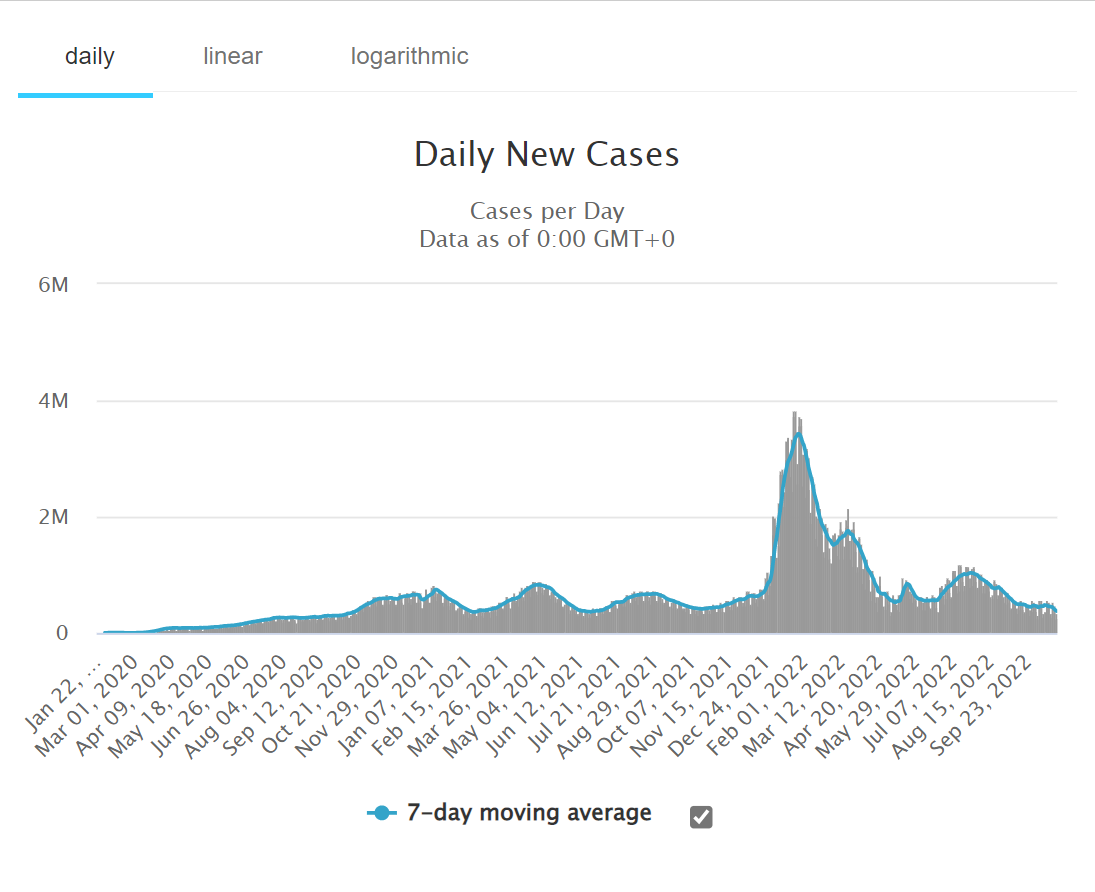
\includegraphics[scale=0.5]{Peta_sebaran.png}
    \caption{Gambar Pertambahan Kasus \covid\ Dunia\cite{a3}.}
    \label{fig:Ch01_denah}
\end{figure}
Sejak kasus \covid\ muncul pada tahun 2019, pandemi ini menyebar dengan cepat hingga terdapat 633.047.720 kasus tercatat pada tanggal 24 Oktober 2022 yang telah dicatat di seluruh negara. Terdapat 6.583.622 kasus kematian dengan 612.165.538 angka pasien yang sembuh. 
Gambar \ref*{fig:Ch01_denah} menunjukkan grafik pertambahan kasus \covid\ setiap hari sejak tanggal 30 Januari 2020 hingga 23 September 2022. Warna hitam menunjukkan angka pertambahan setiap hari sedangkan garis warna biru menunjukkan \textit{7-day moving average} untuk memperlihatkan angka pertambahan kasus baru dan kecepatan pertumbuhannya yang dihitung dari hari data diambil, 3 hari setlah data diambil, dan 3 hari sebelum data diambil. Masih banyak pertambahan kasus yang terjadi hingga saat ini dan kini \covid\ telah menyebar hingga 228 negara. Terkumpul data bahwa untuk kasus aktif saat ini mencapai 14.298.560 dan angka pasien sembuh 618.749.160. Jumlah kematian total hingga saat ini adalah 6.583.622 yang berarti tingkat kematian dari virus ini adalah $1\%$\cite{a4}. 
%https://www.worldometers.info/coronavirus/

\begin{figure}[H]
        \centering
        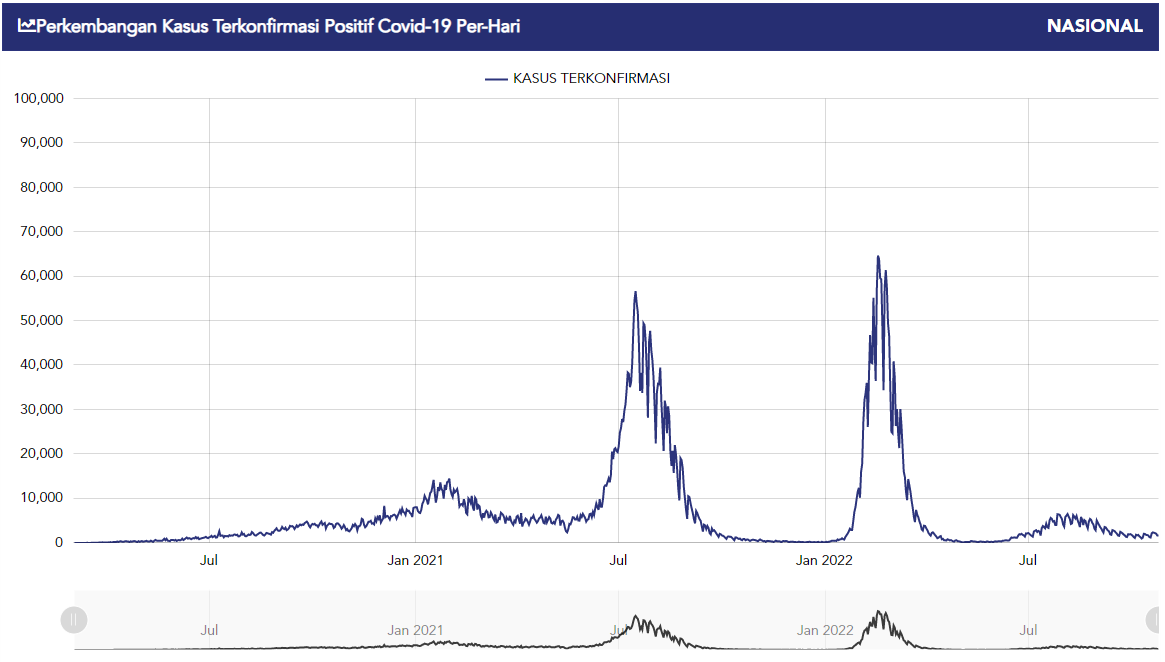
\includegraphics[scale=0.5]{kasus_indo.png}
        \caption{Gambar Perkembangan Kasus \covid\ Indonesia\cite{a1}.}
        \label{fig:Ch01_Indonesia}
    \end{figure}

Pada tanggal 25 November 2022, jumlah kasus tercatat di Indonesia telah mencapai 6.472.664 jiwa dengan jumlah sembuh 6.295.525 dan jumlah meninggal 158.454\cite{a3}. Pada grafik perkembangan yang ditunjukkan Gambar \ref{fig:Ch01_Indonesia}, terlihat pertambahan kasus setiap hari di Indonesia sejak Maret 2021 hingga 25 November 2022. Awal tahun 2022 masih terdapat penambahan yang tinggi hingga 60.000 kasus dalam satu hari. Pada bulan Oktober, jumlah pertambahan kasus berkisar antara 1.000 hingga 2.000 lebih per hari. 

Jumlah kasus terkonfirmasi setiap harinya di Indonesia sudah mulai mengalami penurunan, namun masih banyak pasien yang masih memerlukan perawatan \covid\ dan masih banyak warga yang memerlukan vaksinasi. Hal ini membuktikan bahwa tenaga kesehatan dan fasilitas kesehatan memiliki peran penting dalam kontribusinya menangani \covid. Pemberian bantuan untuk pasien \covid\ dan tenaga kesehatan merupakan salah satu upaya pokok dalam menekan jumlah kasus \covid\ di Indonesia.

\section{Dampak \covid\ terhadap Tenaga Kesehatan}
\label{sec:Dampak_Covid_RS}
Tenaga kesehatan menjadi salah satu garda terdepan dalam penanganan \covid. Meledaknya jumlah pasien COVID-19 membuat berbagai rumah sakit kewalahan karena kekurangan sumber daya salah satunya jumlah tenaga kesehatan yang melayani. Perbedaan yang signifikan antara jumlah pasien dan jumlah tenaga kesehatan ini menyebabkan kelelahan pada tenaga kesehatan karena terlalu banyak bekerja. Tenaga kesehatan juga merupakan pihak yang paling rentan untuk tertular COVID-19 dikarenakan banyaknya kontak langsung terhadap pasien COVID-19. 

\begin{figure}[H]
    \centering
    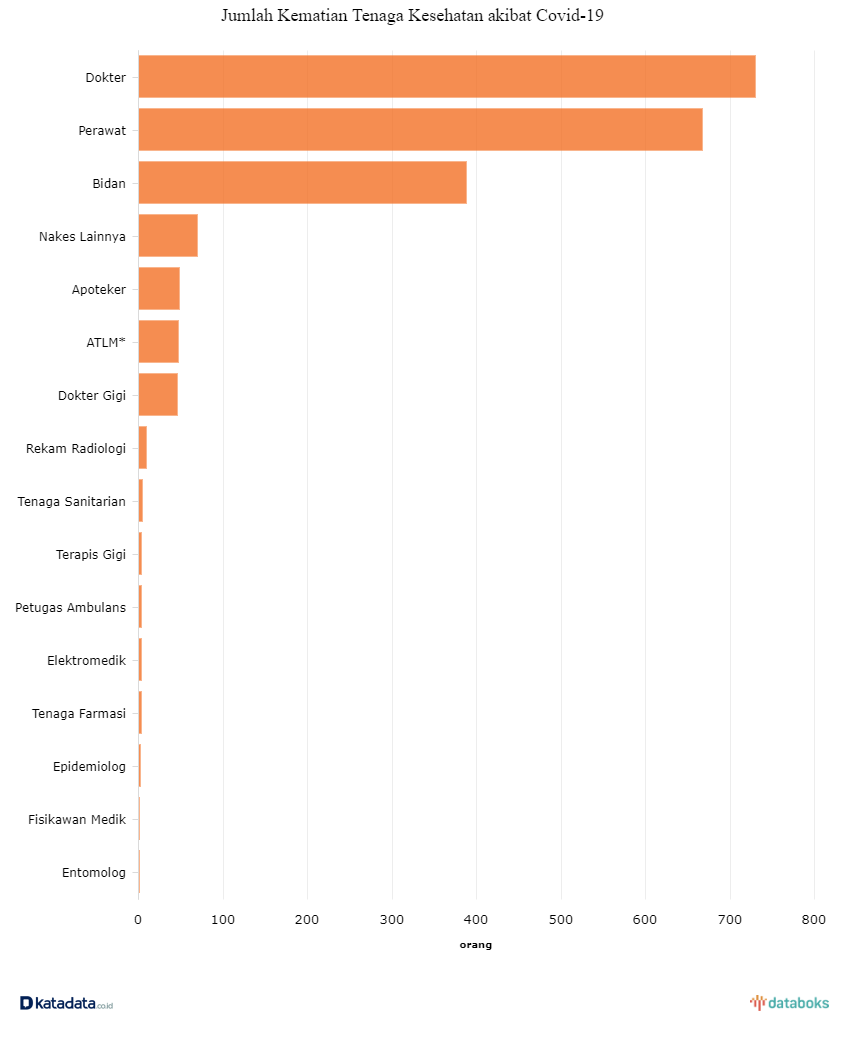
\includegraphics[scale=0.4]{sebanyak-2029-tenaga-kesehatan-meninggal-akibat-covid-19-by-katadata.png}
    \caption{Jumlah Kematian Tenaga Kesehatan Akibat \covid\cite{a6}.}
    \label{fig:Ch01_sebaran_nakes}
\end{figure}

WHO memperkirakan antara 80.000 hingga 180.000 tenaga kesehatan meninggal karena COVID-19 pada periode antara Januari hingga Mei tahun 2020\cite{a5}. Jumlah ini didapatkan dari total 3,45 juta kasus kematian COVID-19 yang dilaporkan ke WHO pada Mei 2021, namun jumlah kasus sebenarnya diduga lebih tinggi 60\% daripada jumlah kematian yang dilaporkan ke WHO. Gambar \ref{fig:Ch01_sebaran_nakes} menunjukkan data yang diperoleh di Indonesia yang menyatakan bahwa pada tanggal 15 September 2021 terdapat 2.029 tenaga kesehatan meninggal akibat \covid\ termasuk 730 dokter dan 667 perawat\cite{a6}.

Pandemi COVID-19 telah memengaruhi tenaga kesehatan secara fisik dan psikologi\cite{a7}.
% https://www.weforum.org/agenda/2020/04/10-april-who-briefing-health-workers-covid-19-ppe-training/
Tenaga kesehatan lebih rentan terjangkit \covid\ daripada masyarakat umum karena lebih sering berkontak dengan pasien. Situasi ini membuat berbagai upaya dibentuk untuk meringankan beban yang ada, termasuk dalam bidang teknologi. Automasi rumah sakit menjadi salah satu inovasi yang dikembangkan untuk mengelola rumah sakit dan fasilitas kesehatan, terutama di saat krisis seperti ini.


% Under such dire circumstances, smart technology adoptions and tech enabled tools can come to the rescue to not only help streamline operations but to also drive efficiency and reduce the burden.

% Hospital automation, or RPA is one such tech innovation that can be of immense help for managing hospitals and healthcare facilities, especially in times of such crisis. From scheduling of doctors and nursing staff, assigning beds or rooms, scheduling OR and consulting room assignments to creating and maintaining a patient treatment record, managing out patients and, especially during COVID, manage the testing and vaccination rush, automate reports and send reminders and appointments for regular patient visits.

\section{Bidang Robotika untuk \covid}
\label{sec:Robotika_covid}
Banyak solusi dan teknologi yang dikembangkan untuk memerangi pandemi ini termasuk dalam bidang robotika. Robot \covid\ dikembangkan dengan tujuan salah satunya untuk menjadi asisten tenaga kesehatan. Robot memiliki keuntungan yaitu dapat bekerja dalam jangka waktu yang lama, melakukan kontak dengan pasien dengan aman, dan meningkatkan efisiensi kerja tenaga kesehatan. Dalam memenuhi tugas ini, robot memerlukan kemampuan dasar untuk mengidentifikasi manusia dan membedakannya dengan benda sekitar. Setelah memiliki kemampuan tersebut, robot kemudian dapat dikembangkan lebih lanjut agar dapat menjalankan berbagai tugas.

\begin{figure}[H]
    \centering
    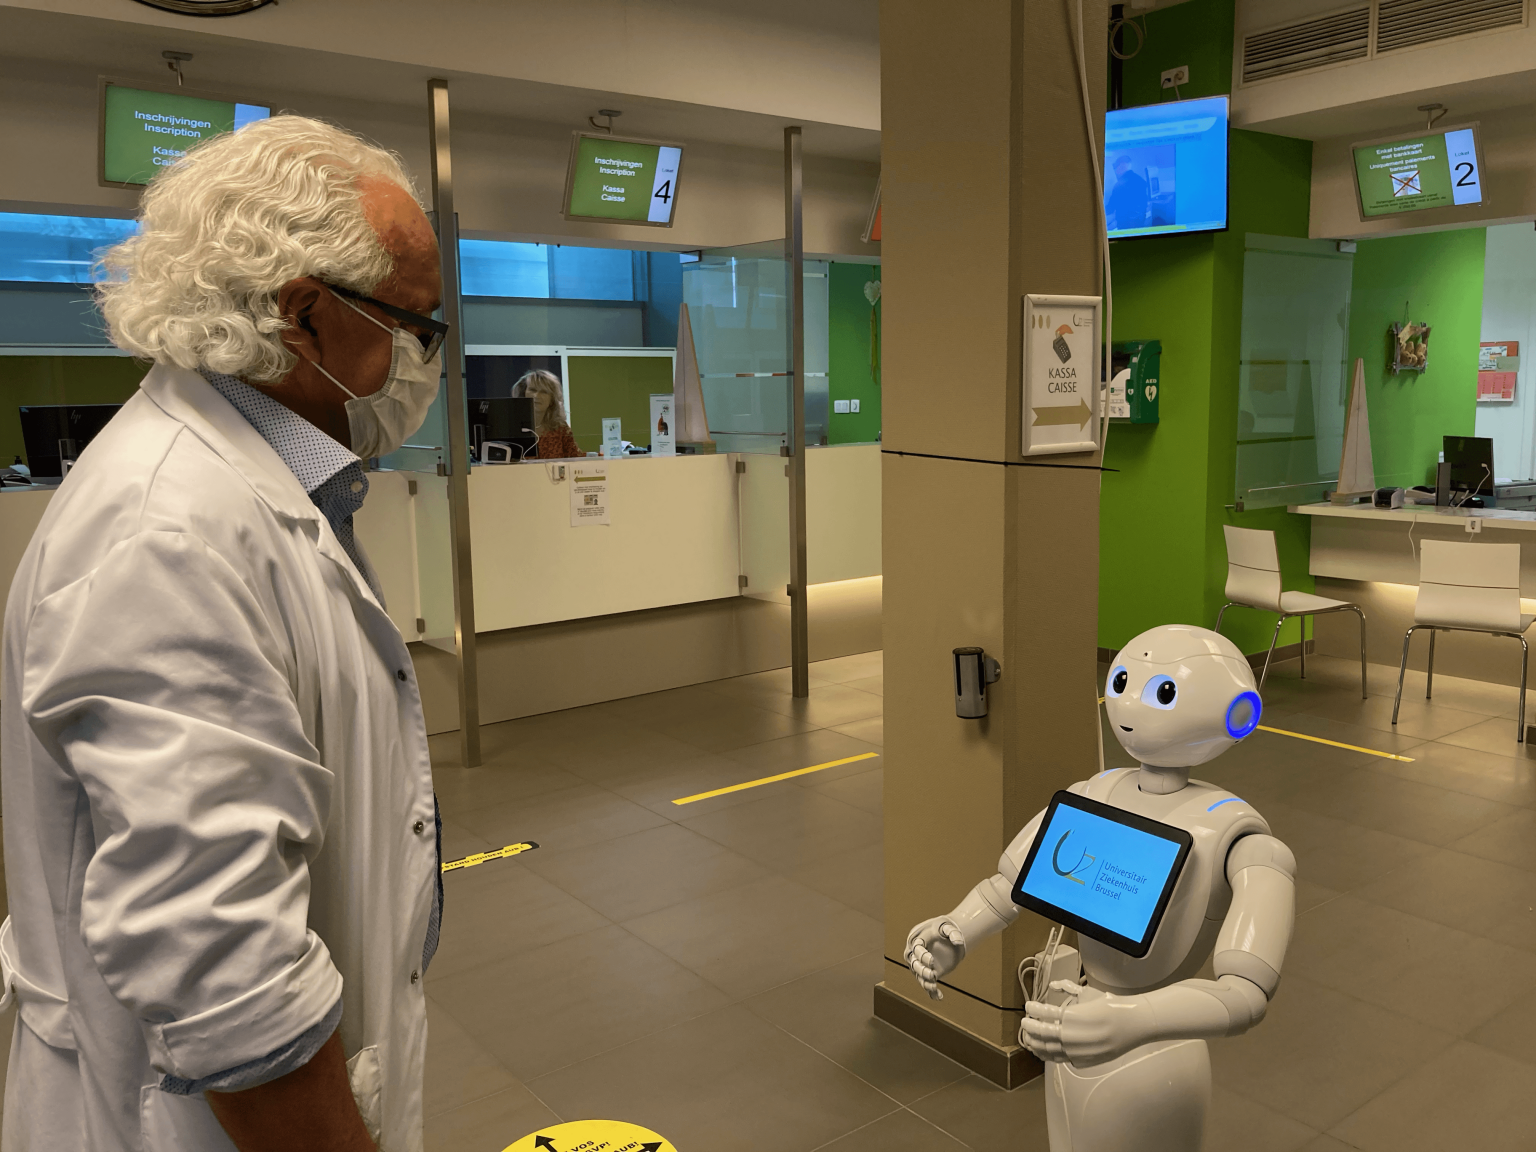
\includegraphics[scale=0.3]{robot_cruzr.png}
    \caption{Robot \textit{Autonomous} CRUZR di Rumah Sakit Belgium\cite{a9}.}
    \label{fig:Ch02_robot_CRUZR}
\end{figure}

Saat ini robot \auto\ juga mulai dikembangkan dalam bidang kesehatan karena dapat memberikan berbagai keuntungan seperti aman, andal, dan mampu untuk memproduksi obat secara efisien\cite{a8}. Gambar \ref{fig:Ch02_robot_CRUZR} merupakan salah satu robot bidang kesehatan yang telah dikembangkan adalah robot CRUZR yang bekerja di \textit{Antwerp University Hospital} di Belgium\cite{a9}. Robot ini mempunyai tugas untuk menyapa pasien, mengecek suhu tubuh dan masker pasien, kemudian mengantar pasien ke ruang yang ingin dituju. Robot ini beroperasi secara mandiri tanpa operator manusia. Hal ini memberikan kelebihan yaitu berkurangnya kontak antara tenaga kesehatan dengan pasien pada masa pandemi \covid\ ini.

\begin{figure}[H]
    \centering
    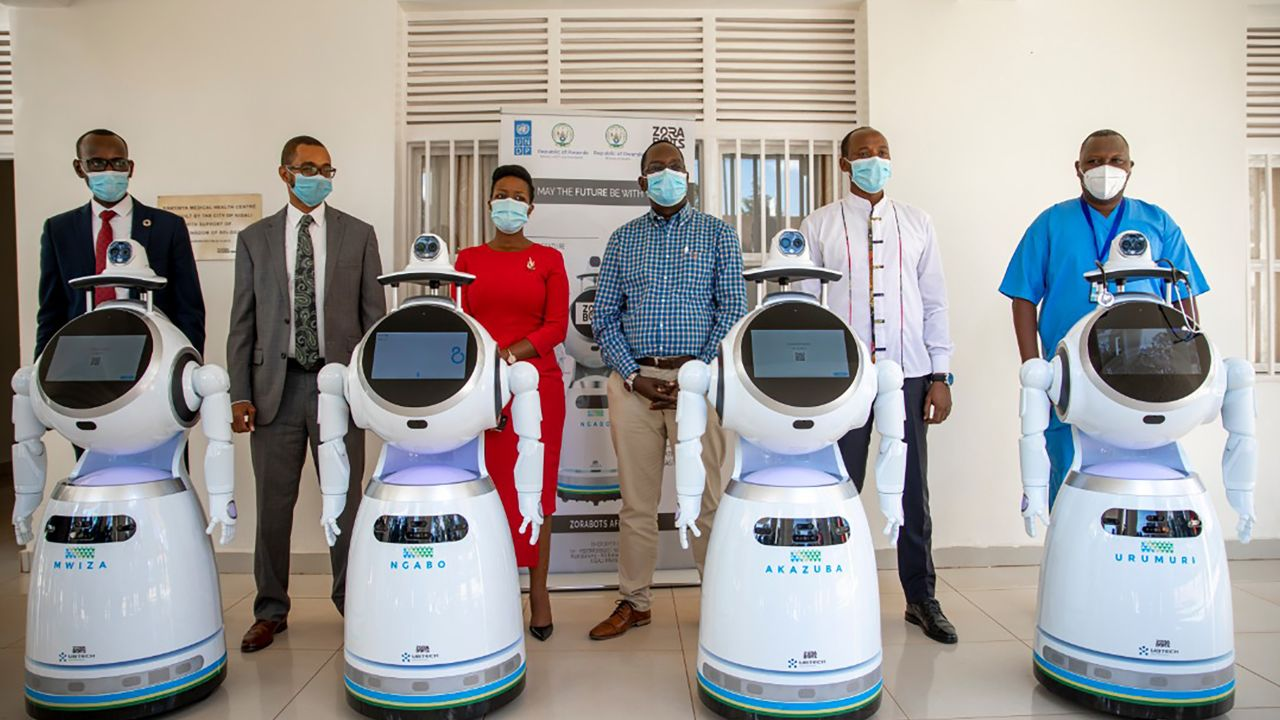
\includegraphics[scale=0.26]{robot_rwanda.jpg}
    \caption{Robot Pelayan Pasien \covid\ di Afrika \cite{a10}.}
    \label{fig:Ch02_robot_rwanda}
\end{figure}
    

Gambar \ref*{fig:Ch02_robot_rwanda} menunjukkan robot-robot pelayan pasien \covid\ dari United Nations Development Program (UNDP) untuk Kanyinya sebagai robot pelayan pasien \covid\ di Kigali, Afrika. Robot-robot tersebut bernama Akazuba, Ikirezi, Mwiza, Ngabo, and Urumuri yang bertugas untuk membantu perawatan pasien. Robot-robot ini dapat melakukan pemindaian suhu massal, pemantauan status pasien, dan penyimpanan rekam medis pasien \covid. Robot juga memiliki kemampuan menangkap data suara dan visual pasien dan dapat memberi tahu petugas kesehatan tentang kelainan yang terdeteksi.
% https://edition.cnn.com/2020/05/25/africa/rwanda-coronavirus-robots/index.html

Pada proyek \textit{capstone} ini dirancang sistem untuk mengembangkan kemampuan robot \covid\ sehingga dapat mengidentifikasi objek manusia dan benda untuk robot \covid. Robot nantinya secara otomatis mampu membedakan objek manusia dengan benda di sekitarnya dari bacaan sensor yang ditanam pada robot. Adanya sistem pendeteksi manusia dan benda ini dapat memberikan solusi untuk pengembangan berbagai kemampuan robot seperti \textit{tracking}, membantu menjadi asistensi tenaga kesehatan, membantu melayani pasien, menggantikan beberapa tugas tenaga kesehatan, hingga menjaga kenyamanan dan keamanan lingkungan rumah sakit. Dengan demikian, robot dapat ikut membantu mengurangi beban kerja tenaga kesehatan dan meningkatkan kualitas pelayanan \covid.

% Bab-bab dalam dokumen C501 ini terdiri dari 11 bab. Bab pertama menjelaskan latar belakang permasalahan yang diangkat. Bab kedua menguraikan dasar teori pendukung yang diperlukan proyek ini. Bab ketiga akan mengenalkan berbagai metode yang dapat menyelesaikan permasalahan. Bab keempat berisi pemodelan matematika dari permasalahan proyek ini. Bab kelima menjelaskan pemilihan metode yang paling tepat untuk menyelesaikan masalah. Bab keenam berisi jenis luaran yang diinginkan beserta spesifikasinya. Bab tujuh menunjukkan batas-batas permasalahan yang diangkat. Bab delapan berisi rancangan umum sistem. Bab sembilan berisi rencana rangka anggaran dan rencana jadwal kegiatan proyek. Bab sepuluh memperlihatkan simulasi awal proyek ini. Bab terakhir yaitu bab sebelas memuat kesimpulan dari rancangan sistem yang akan dibuat dan diimplementasikan.
